\section{Atividades}

\subsection{Consulta WHOIS}

\begin{figure}[H]
\centering
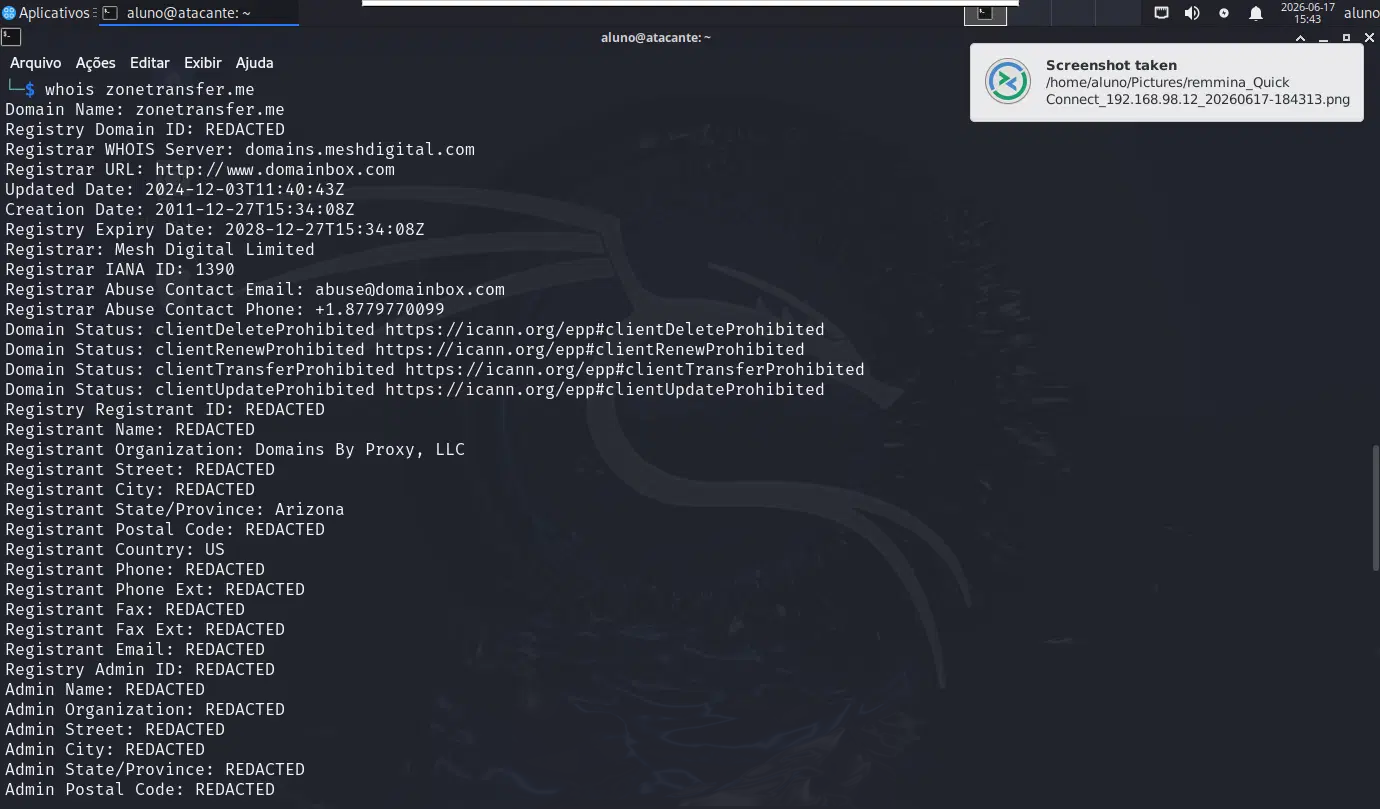
\includegraphics[width=0.95\textwidth]{./fig/whois.png}
\caption{Resultado da consulta WHOIS.}
\end{figure}

A consulta WHOIS permitiu obter informações públicas relacionadas ao registro
do domínio analisado, incluindo servidores DNS, entidade registradora e dados
administrativos disponibilizados pelo registro.

\subsection{Enumeração de Subdomínios com DNSenum}

\begin{figure}[H]
\centering
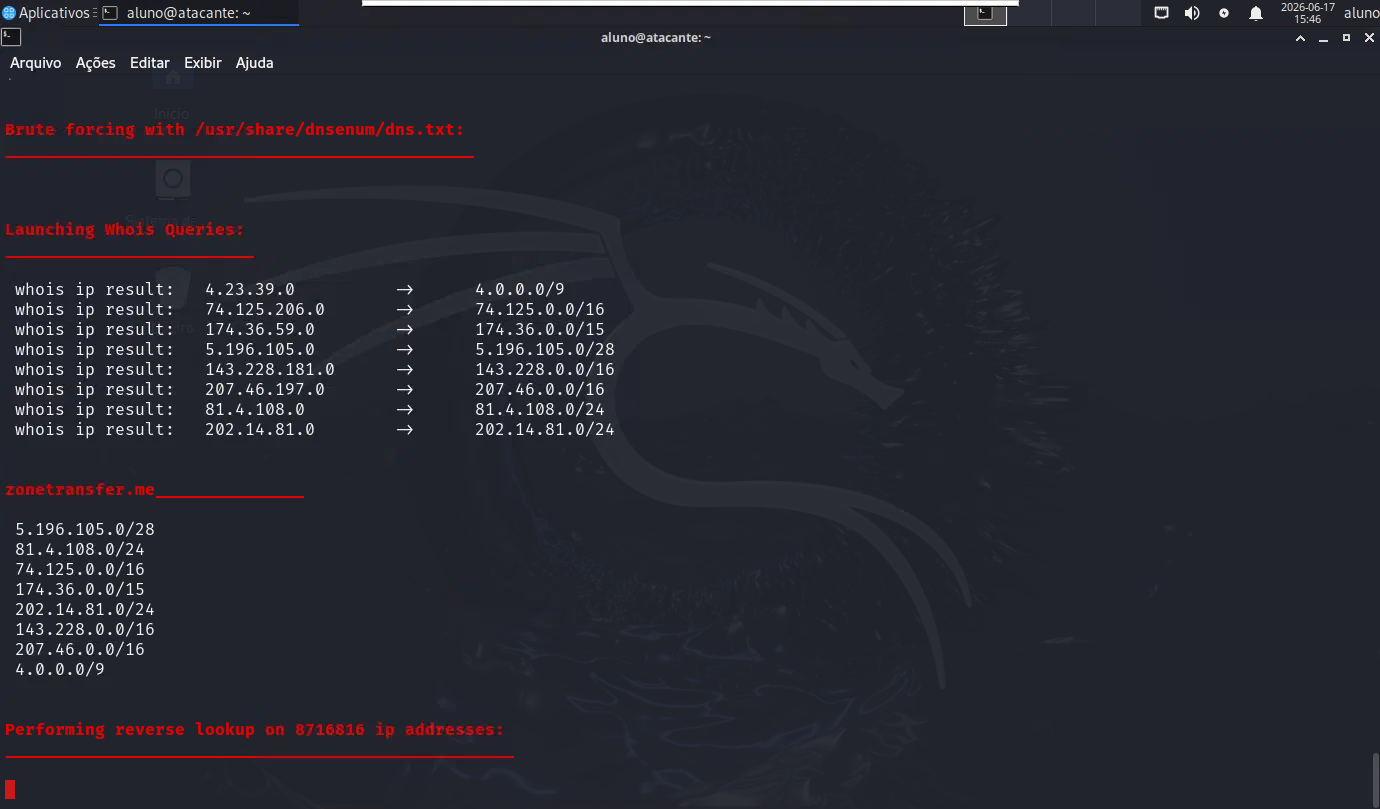
\includegraphics[width=0.95\textwidth]{./fig/dnsenum.png}
\caption{Resultado da enumeração utilizando DNSenum.}
\end{figure}

A ferramenta DNSenum foi utilizada para identificar subdomínios associados ao
alvo por meio de consultas DNS e técnicas de força bruta.

\newpage
\subsection{Enumeração de Subdomínios com DNSRecon}

\begin{figure}[H]
\centering
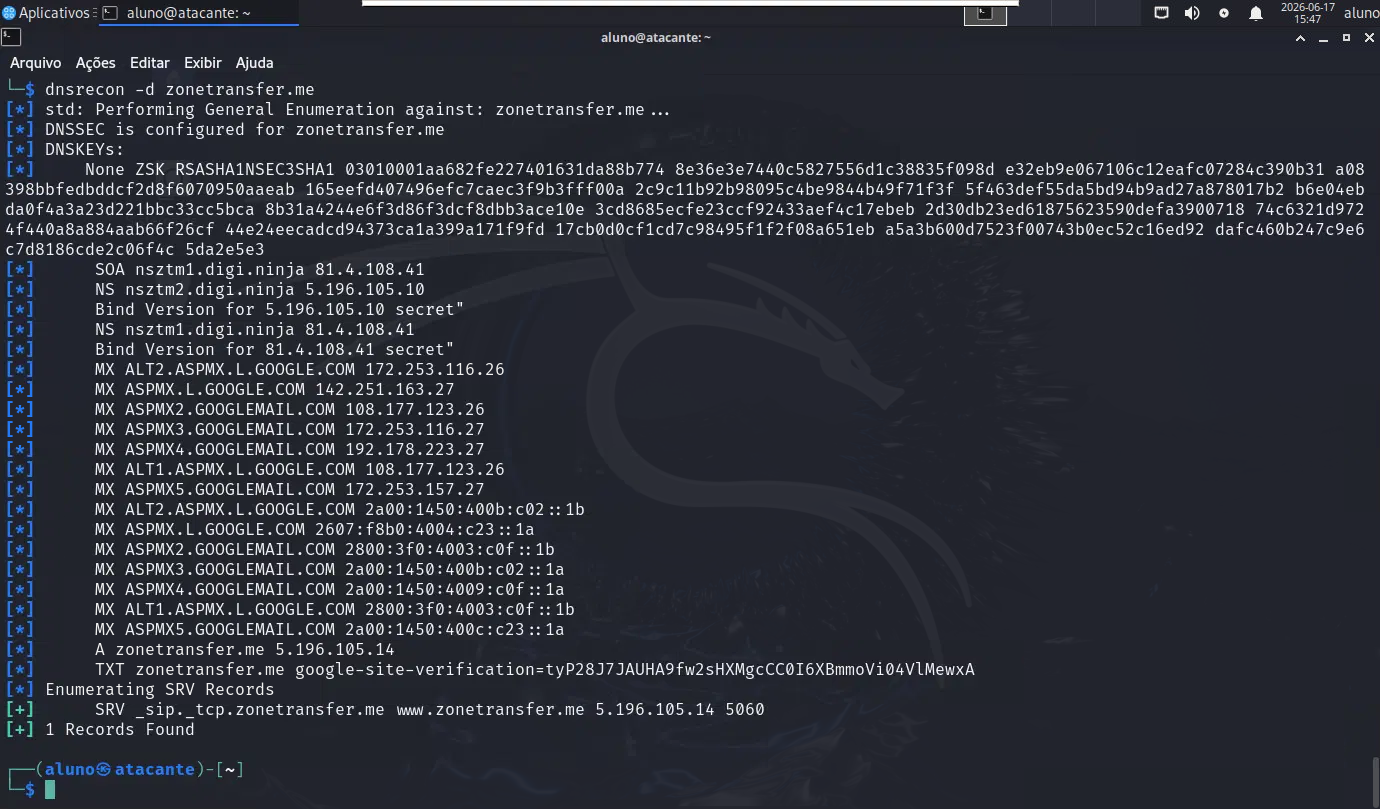
\includegraphics[width=0.95\textwidth]{./fig/dnsrecon.png}
\caption{Resultado da enumeração utilizando DNSRecon.}
\end{figure}

O DNSRecon permitiu identificar registros DNS e possíveis subdomínios
relacionados ao domínio analisado.

\newpage
\subsection{Enumeração de Subdomínios com DNSMap}

\begin{figure}[H]
\centering
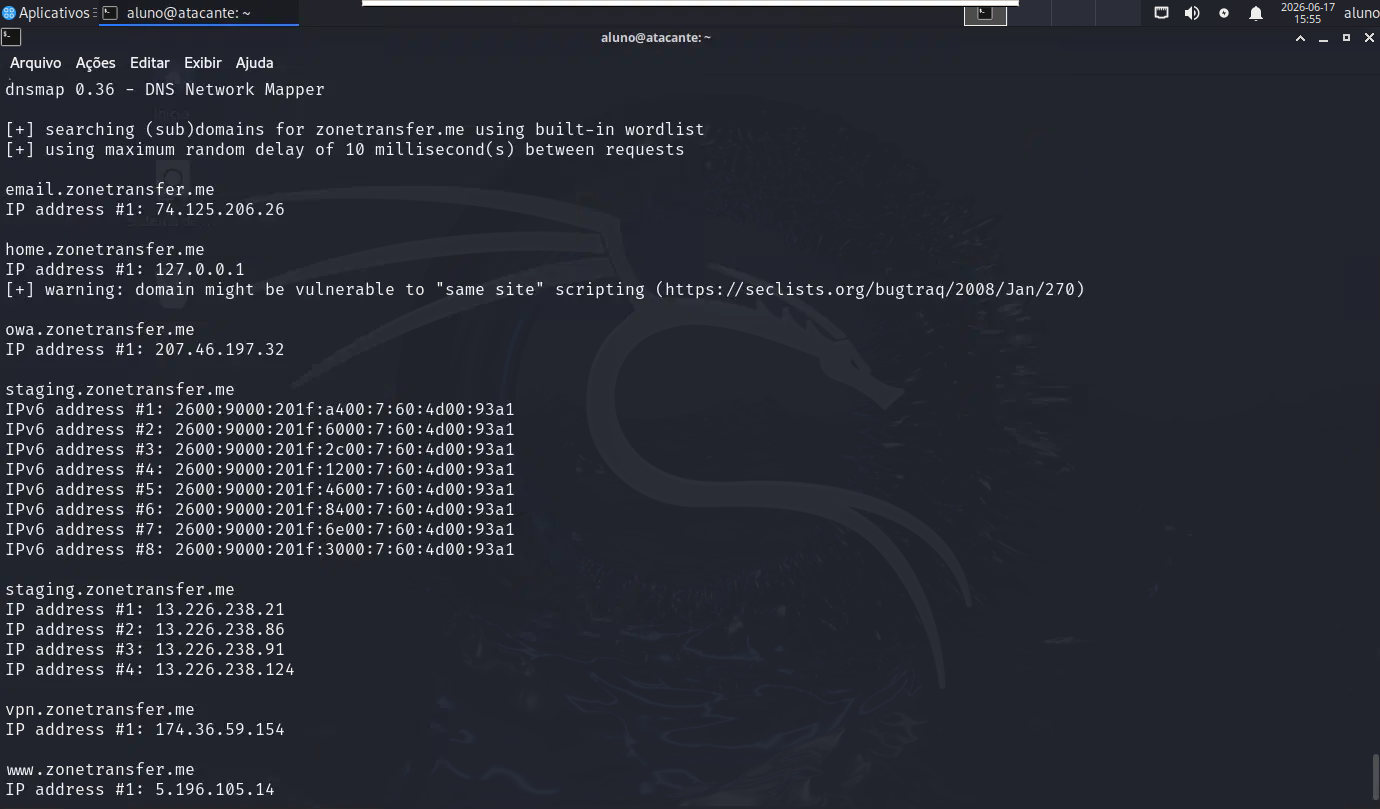
\includegraphics[width=0.95\textwidth]{./fig/dnsmap.png}
\caption{Resultado da enumeração utilizando DNSMap.}
\end{figure}

A ferramenta DNSMap realizou tentativas de descoberta de subdomínios por meio
de listas de nomes comuns, auxiliando no mapeamento da infraestrutura.

\subsection{Resolução Reversa com dig}

\begin{figure}[H]
\centering
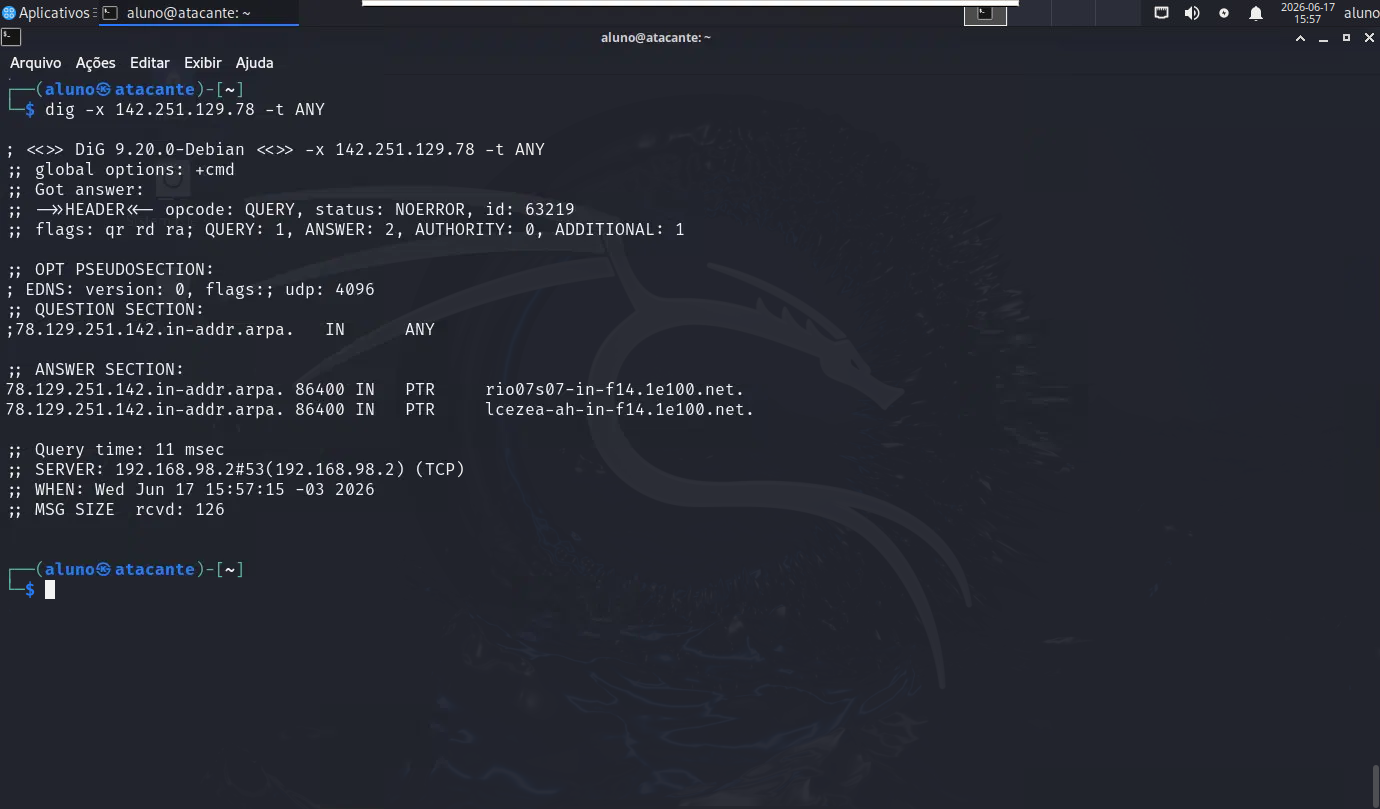
\includegraphics[width=0.95\textwidth]{./fig/dig.png}
\caption{Resultado da consulta reversa utilizando dig.}
\end{figure}

A consulta reversa permitiu verificar a existência de registros PTR associados
ao endereço IP analisado.

\subsection{Resolução Reversa com nslookup}

\begin{figure}[H]
\centering
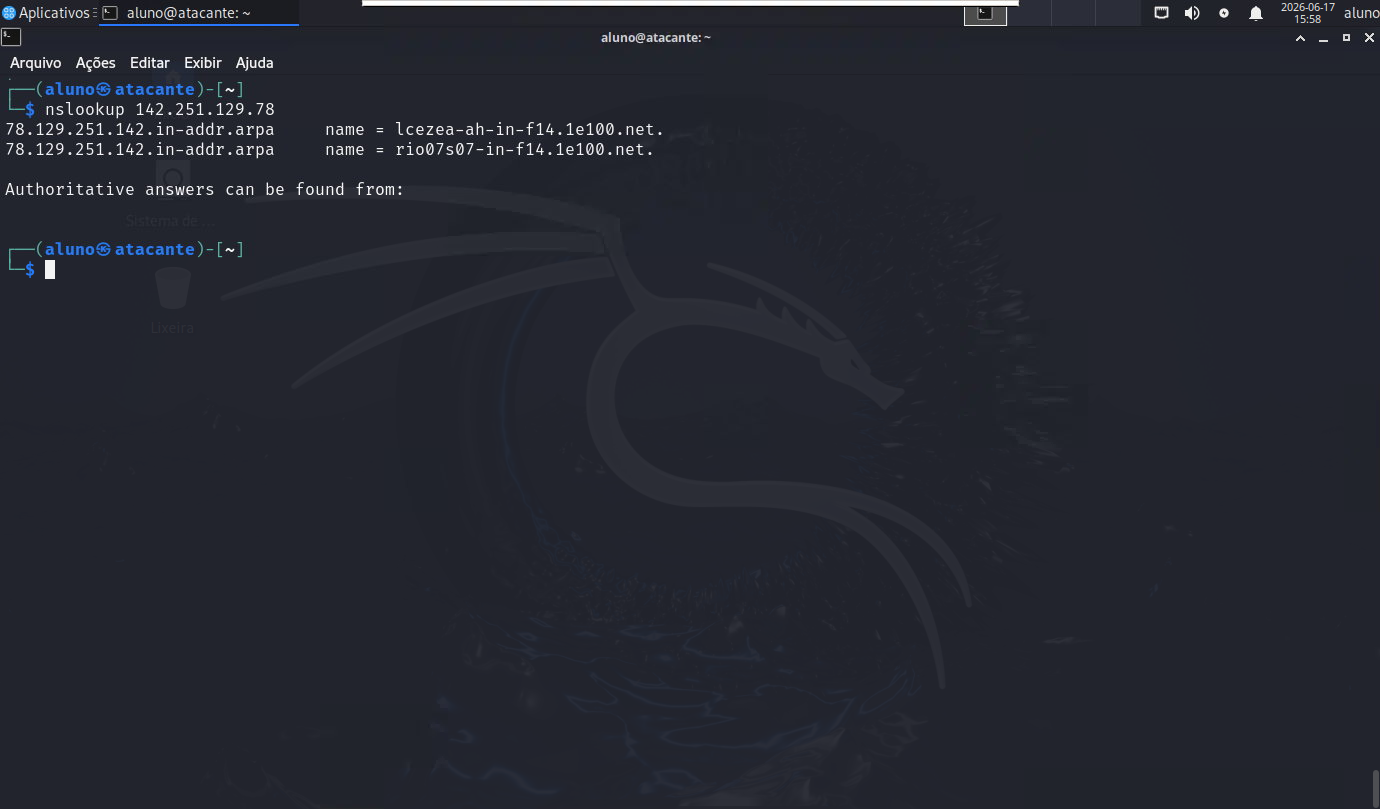
\includegraphics[width=0.95\textwidth]{./fig/nslookup.png}
\caption{Resultado da consulta reversa utilizando nslookup.}
\end{figure}

O comando nslookup foi utilizado para validar as informações obtidas por meio
da consulta reversa DNS.

\subsection{Teste de Transferência de Zona}

\begin{figure}[H]
\centering
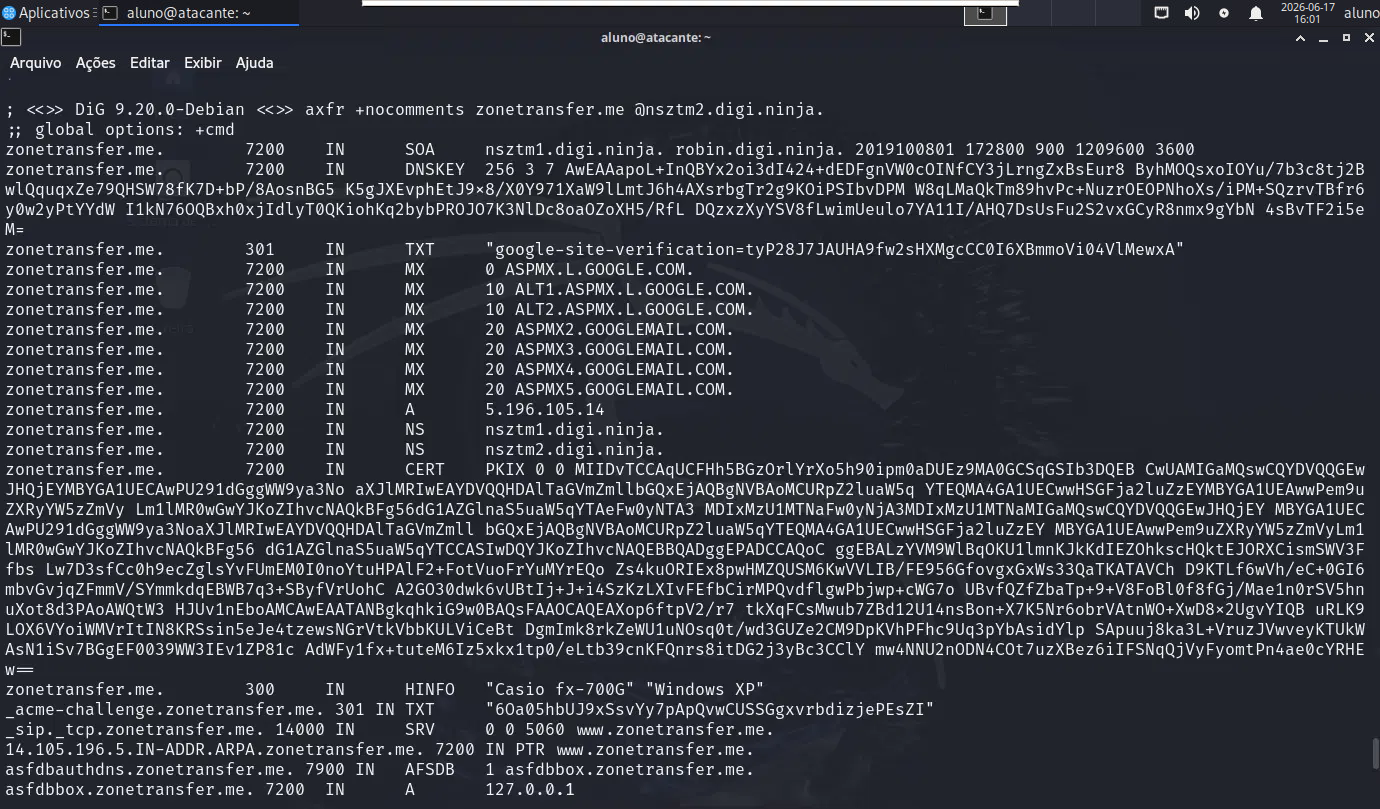
\includegraphics[width=0.95\textwidth]{./fig/zonetransfer.png}
\caption{Resultado do teste de transferência de zona DNS.}
\end{figure}

O teste teve como objetivo verificar se os servidores DNS permitiam a
transferência completa dos registros da zona, o que poderia expor informações
sensíveis da infraestrutura.

\subsection{Consulta de Certificados com CRT.SH}

\begin{figure}[H]
\centering
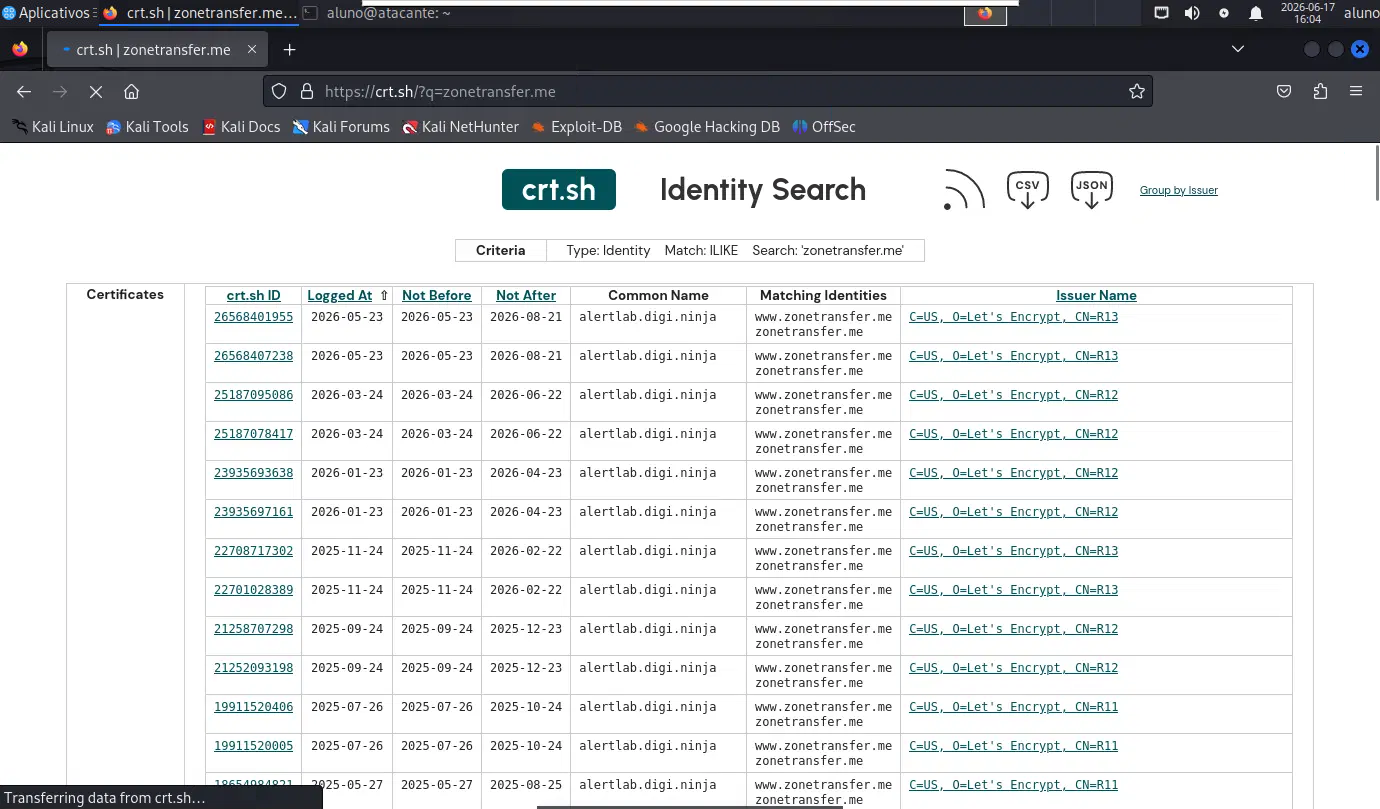
\includegraphics[width=0.95\textwidth]{./fig/crtsh.png}
\caption{Resultado da consulta no CRT.SH.}
\end{figure}

A plataforma CRT.SH foi utilizada para identificar certificados digitais
emitidos para o domínio e possíveis subdomínios associados.

\newpage
\subsection{Enumeração com Amass}

\begin{figure}[H]
\centering
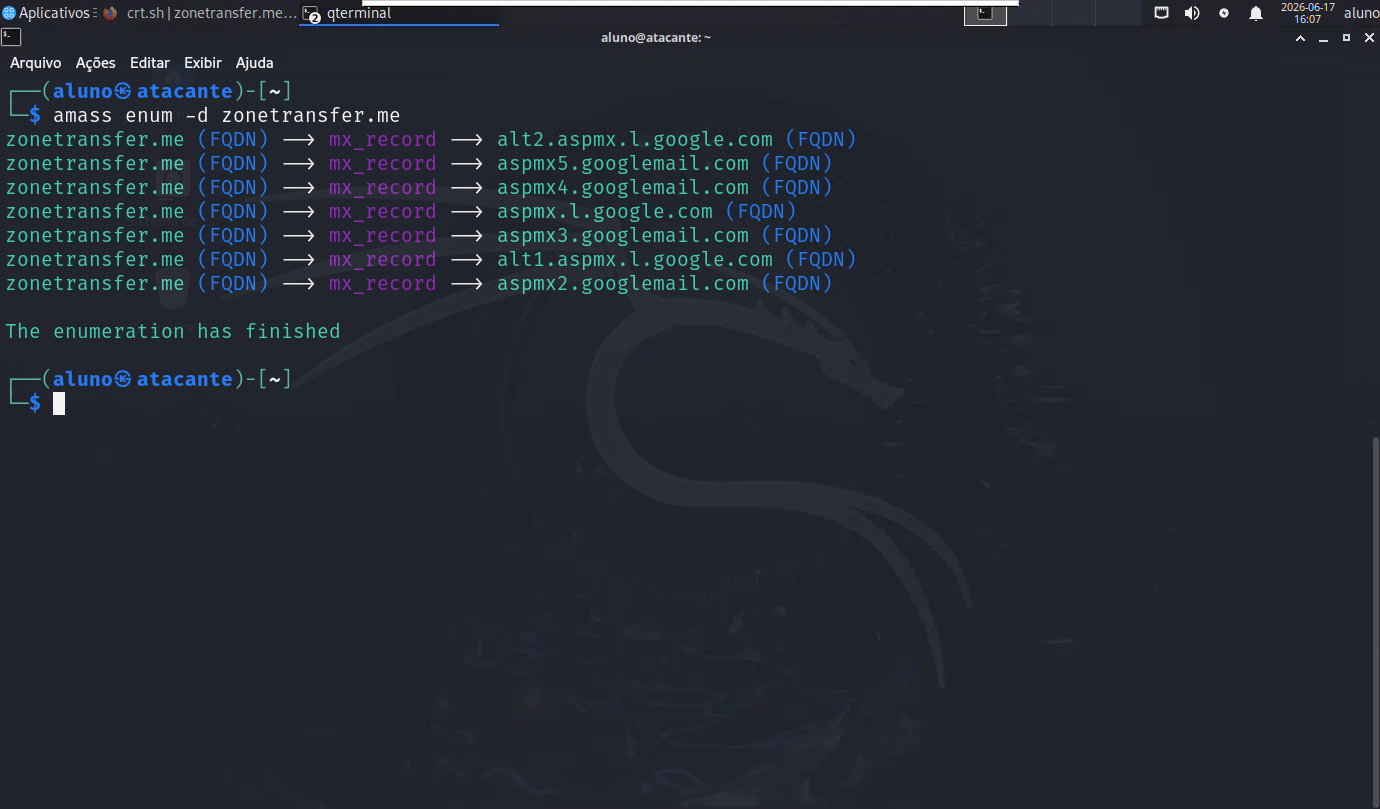
\includegraphics[width=0.95\textwidth]{./fig/amass.png}
\caption{Resultado da enumeração utilizando Amass.}
\end{figure}

O Amass realizou a correlação de informações provenientes de diversas fontes
abertas, ampliando a visibilidade sobre a superfície de ataque do alvo.
